\documentclass[12pt,a4paper]{article}

\usepackage[utf8]{inputenc}
\usepackage[T1]{fontenc}
\usepackage[italian]{babel}
\usepackage{graphicx}
\usepackage{longtable}
\usepackage{array}
\usepackage{geometry}
\usepackage[table]{xcolor}
\usepackage{fancyhdr}
\usepackage{titlesec}
\usepackage{hyperref}
\usepackage{float}
\usepackage{caption}
\usepackage{enumitem}

\geometry{margin=2.5cm}
\setlength{\parindent}{0pt}
\setlength{\parskip}{\baselineskip}
\captionsetup[table]{position=bottom}

\definecolor{lightblue}{RGB}{10,160,255}
\definecolor{unipablue}{RGB}{0,70,127}

\hypersetup{
    colorlinks=true,
    linkcolor=unipablue,
    urlcolor=unipablue,
    pdftitle={SDD},
    pdfauthor={Simone Sottile, Matteo Duca, Giuseppe Giacomarra, Gilberto Mogavero}
}

\pagestyle{fancy}
\setlength{\headheight}{14.5pt}
\fancyhf{}
\fancyhead[L]{\small\textit{AFAM Connect}}
\fancyhead[R]{\small\textit{SDD}}
\fancyfoot[C]{\thepage}
\renewcommand{\headrulewidth}{0.4pt}
\fancypagestyle{plain}{
    \fancyhf{}
    \fancyfoot[C]{\thepage}
    \renewcommand{\headrulewidth}{0pt}
}

\titleformat{\section}
  {\normalfont\Large\bfseries\color{unipablue}}
  {\thesection}{1em}{}[{\color{unipablue}\titlerule[0.5pt]}]

\titleformat{\subsection}
  {\normalfont\large\bfseries}
  {\thesubsection}{1em}{}

\titleformat{\paragraph}[block]
  {\normalfont\normalsize\bfseries}
  {\theparagraph}{1em}{}

\titleformat{\subparagraph}[block]
  {\normalfont\normalsize\bfseries}
  {\thesubparagraph}{1em}{}

\titlespacing*{\paragraph}{0pt}{1.25em}{0.5em}
\titlespacing*{\subparagraph}{0pt}{1em}{0.4em}

\setcounter{secnumdepth}{5}
\setcounter{tocdepth}{5}

\newcommand{\spaziocontenuto}{\mbox{}\par\vspace{1.2cm}}

\begin{document}

\pagenumbering{arabic}
\setcounter{page}{1}
\begin{minipage}[t][\dimexpr\textheight-1cm\relax][t]{\textwidth}
    \thispagestyle{plain}
    \centering

    
\includegraphics[width=0.25\textwidth]{logo-unipa.png}

    \vspace{0.5cm}
    {\large\textsc{Universit\`a degli Studi di Palermo}\par}
    \vspace{0.15cm}
    {\small\textsc{Dipartimento di Ingegneria --- A.A. 2025/2026}\par}

    \vspace{1.8cm}

    \resizebox{\textwidth}{!}{%
        \textbf{\color{unipablue}System Design Document}%
    }

    \vspace{0.8cm}
    
\includegraphics[width=0.5\textwidth]{pdf/logoIDS-transparent.png}

    \vfill

    {\large\textbf{Gruppo di lavoro}\par}
    \vspace{0.4cm}
    {\large
        Simone Sottile\\
        Matteo Duca\\
        Giuseppe Giacomarra\\
        Gilberto Mogavero
    \par}

    \vspace{1.5cm}
\end{minipage}
\newpage

\tableofcontents
\newpage

\section{Obiettivo del sistema}
L'obiettivo del sistema e' la progettazione di una piattaforma per la gestione dell'identita' digitale degli studenti appartenenti alle istituzioni AFAM. Il sistema deve fornire uno strumento digitale unico che permetta a ciascuno studente di rappresentare il proprio percorso artistico e formativo in modo moderno ed efficace, includendo non solo i dati anagrafici e accademici, ma anche la produzione artistica come registrazioni audio, video, spartiti e curriculum.

Il fine principale e' consentire agli studenti di organizzare i propri contenuti in maniera flessibile, decidere autonomamente cosa rendere visibile e condividere il profilo, o parti di esso, con soggetti esterni come commissioni di audizione, enti valutatori o collaboratori. La condivisione avviene tramite collegamenti temporizzati o codici di sblocco, mantenendo il controllo sui materiali e permettendo allo studente di verificare le effettive visualizzazioni.

\section{Architettura software attuale}
Attualmente non esiste una soluzione software unificata per questa specifica esigenza all'interno delle istituzioni AFAM. Gli studenti si trovano quindi a dover presentare il proprio profilo in modo manuale, utilizzando documenti separati, file sparsi e materiali inviati tramite email o altri canali esterni alla piattaforma.

Questo approccio frammentato genera difficolta' nel mantenere la coerenza, l'aggiornamento e il controllo su cio' che viene condiviso in contesti critici quali audizioni, candidature, concorsi o collaborazioni. Inoltre, non e' presente una repository centralizzata dei contenuti artistici: i materiali non sono organizzati in categorie persistenti, non dispongono di uno stato di privacy gestito dal sistema e non sono associati a meccanismi strutturati di tracciamento, revoca o scadenza delle condivisioni.

\section{Architettura software proposta}
L'architettura software proposta introduce una piattaforma centralizzata basata su una repository applicativa dei dati e dei contenuti degli studenti. Tale repository e' gestita tramite il DBMS e conserva in modo persistente le informazioni anagrafiche, il background artistico, le categorie, i file multimediali, i link di condivisione e i codici di sblocco.

Il sistema viene organizzato in sottosistemi applicativi specializzati, ciascuno responsabile di un gruppo coerente di funzionalita': Gestione Studente, Gestione Autenticazione, Gestione Condivisione, Consulta e Gestione Operazioni Automatiche. La boundary DBMS rappresenta il punto di accesso ai dati persistenti e fornisce alle componenti di controllo i metodi necessari per recuperare, salvare e aggiornare gli oggetti di dominio.

\subsection{Panoramica}
Il software sara' installato su un nodo di un'infrastruttura AFAM e sara' progettato per gestire in modo affidabile i dati degli studenti e i contenuti multimediali caricati. L'architettura prevede un sistema con accesso sicuro tramite credenziali personali gestibili in autonomia dallo studente, includendo funzioni di base per la gestione dell'account come il recupero della password.

L'interfaccia utente dovra' essere chiara, intuitiva e orientata alla facilita' d'uso, in modo da adattarsi anche a utenti non esperti dal punto di vista tecnico e provenienti da ambiti artistici. Dal punto di vista architetturale, la soluzione dovra' poter essere estesa in futuro verso l'utilizzo di sistemi di identita' digitale nazionali ed europei, come SPID ed eIDAS, tenendo conto dei relativi principi di affidabilita' e sicurezza.

In via opzionale, la progettazione potra' valutare soluzioni per una futura interazione con sistemi analoghi utilizzati da altre istituzioni AFAM, mantenendo comunque il controllo locale sulla repository dei dati e dei contenuti.

\subsection{Requisiti minimi per l'utilizzo del software proposto}
Per funzionare correttamente e rispettare le specifiche minime del progetto, il sistema richiede:

\begin{itemize}
    \item \textbf{Nodo infrastrutturale AFAM:} un ambiente server su cui installare il sistema e archiviare in modo sicuro i dati personali e i materiali artistici, che possono rappresentare opere originali degli studenti.
    \item \textbf{Connessione di rete:} una rete stabile che permetta agli studenti l'accesso sicuro tramite credenziali, la generazione di link esterni e il funzionamento del sistema di tracciamento delle visualizzazioni.
    \item \textbf{DBMS relazionale:} un sistema di gestione dei dati persistenti per memorizzare studenti, background artistico, categorie, contenuti, link, codici e relative associazioni.
    \item \textbf{Storage dei contenuti:} uno spazio di archiviazione per i file audio, video e PDF caricati dagli studenti, collegato ai record presenti nel DBMS tramite il percorso fisico del file.
    \item \textbf{Meccanismi di privacy e tutela dei contenuti:} funzioni integrate per controllare la visibilita' dei file, limitarne la consultazione e riservare l'accesso a specifici destinatari tramite link temporizzati o codici di sblocco.
\end{itemize}

\subsection{Decomposizione in sottosistemi}
La decomposizione del sistema segue la seguente suddivisione. I sottosistemi individuati sono i seguenti:

\begin{figure}[H]
    \centering
    
\includegraphics[width=\textwidth,height=0.78\textheight,keepaspectratio]{pdf/asta/decomposizioneSottosistemi.pdf}
    \caption{Decomposizione del sistema in sottosistemi}
    \label{fig:decomposizione_sottosistemi}
\end{figure}

\newpage

\begin{itemize}
    \item \textbf{Gestione Studente:} raccoglie le funzionalita' con cui lo studente amministra il proprio profilo, il portfolio e i contenuti caricati. Include la gestione dei dati personali e artistici, la creazione delle categorie, la selezione delle tipologie di file, l'upload, la modifica, l'eliminazione e la gestione della privacy dei contenuti.
    \item \textbf{Gestione Autenticazione:} gestisce l'accesso alla piattaforma e le operazioni collegate all'account. Comprende login, registrazione, recupero password, logout e l'interazione con eventuali boundary dedicate all'identita' digitale.
    \item \textbf{Gestione Condivisione:} governa la condivisione dei contenuti dello studente. Comprende la selezione dei file da condividere, la generazione e visualizzazione dei link temporizzati, la generazione dei codici di sblocco, la selezione dei contenuti privati e la revoca dei permessi di accesso.
    \item \textbf{Consulta:} consente la consultazione dei profili e dei contenuti autorizzati. Include la ricerca dello studente, la visualizzazione del profilo, la consultazione dei contenuti pubblici, lo sblocco dei contenuti privati tramite codice e la visualizzazione dei contenuti condivisi tramite link.
    \item \textbf{Gestione Operazioni Automatiche:} contiene le funzionalita' eseguite automaticamente dal sistema, in particolare il controllo temporale sulla validita' dei link di condivisione e l'aggiornamento del relativo stato quando risultano scaduti.
\end{itemize}

\newpage

\subsection{Suddivisione degli oggetti all'interno dei sottosistemi e dei componenti}

\textbf{Gestione Studente:}

\begin{figure}[H]
    \centering
    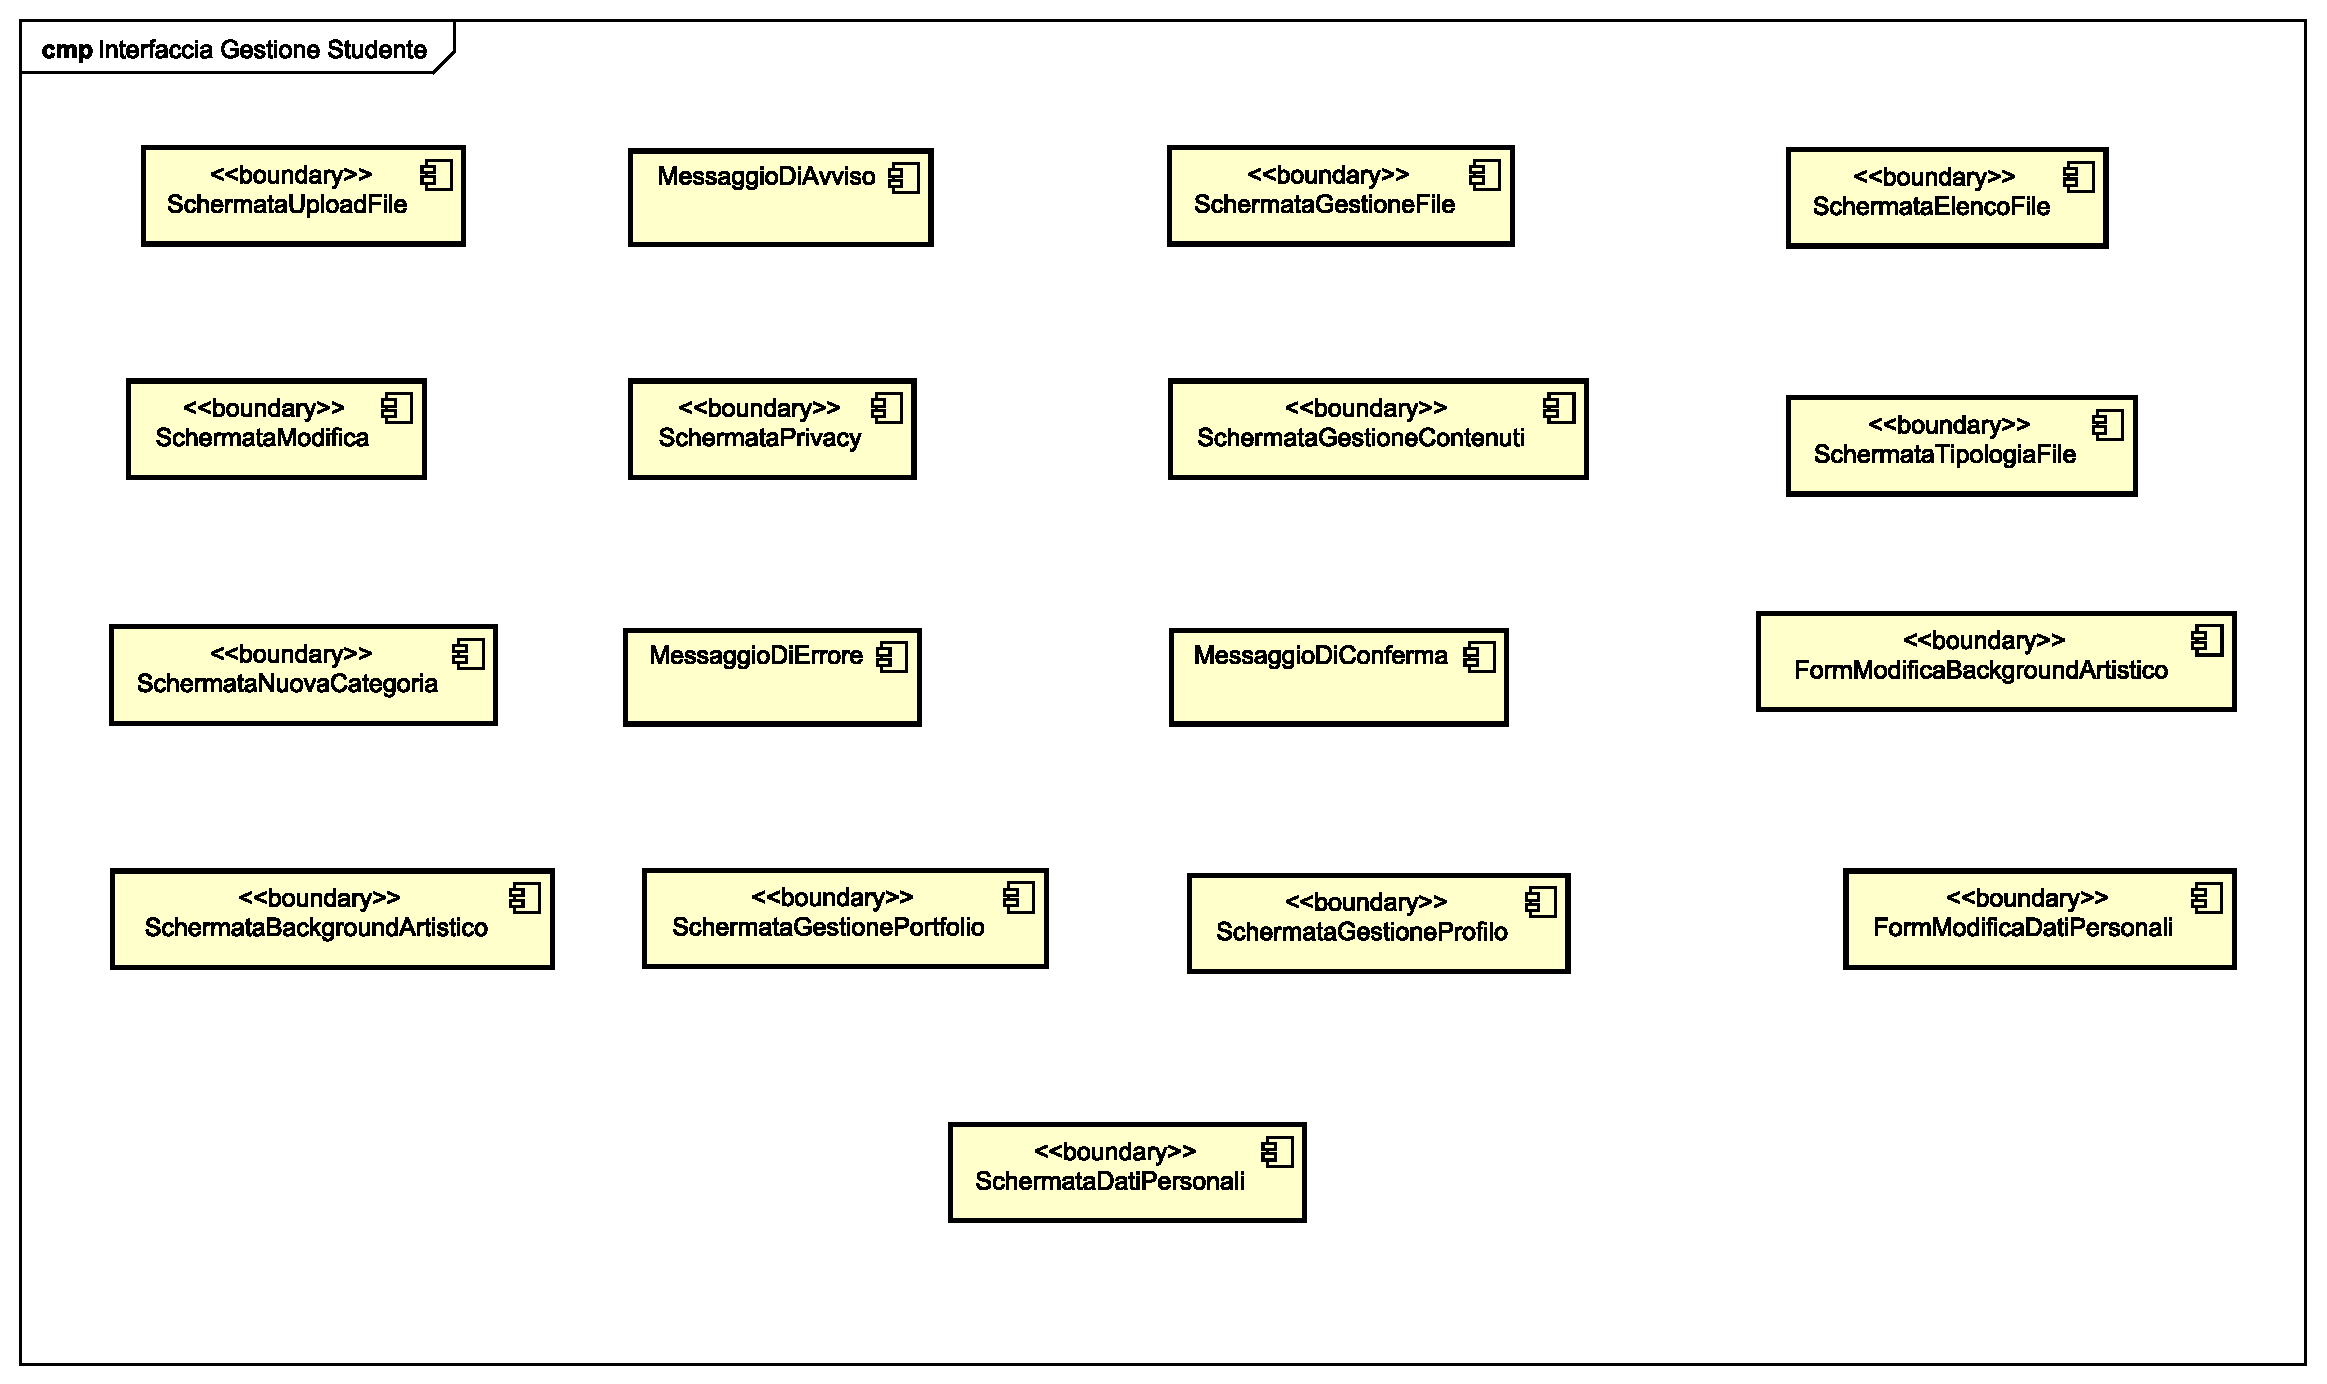
\includegraphics[width=\textwidth,height=0.72\textheight,keepaspectratio]{pdf/asta/gestioneStudente_Interfaccia_Gestione_Studente.pdf}
    \caption{Interfaccia del sottosistema Gestione Studente}
    \label{fig:interfaccia_gestione_studente}
\end{figure}

\begin{figure}[H]
    \centering
    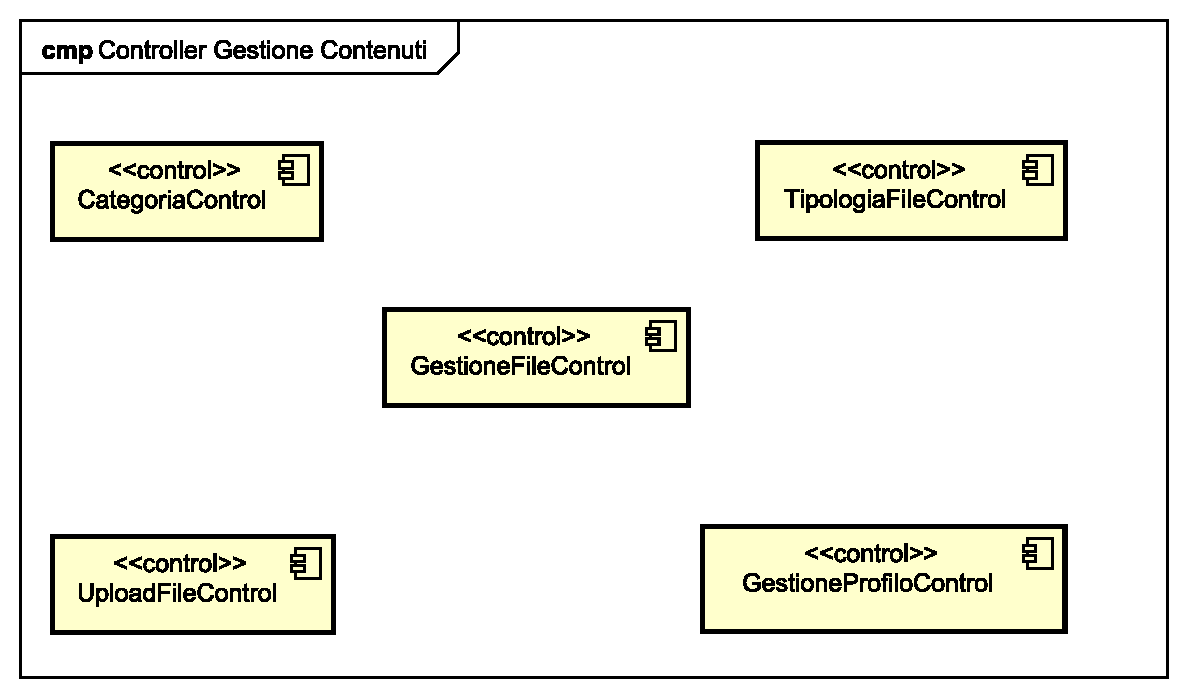
\includegraphics[width=\textwidth,height=0.72\textheight,keepaspectratio]{pdf/asta/gestioneStudente_Controller_Gestione_Contenuti.pdf}
    \caption{Controller del sottosistema Gestione Studente}
    \label{fig:controller_gestione_studente}
\end{figure}

\newpage

\textbf{Gestione Autenticazione:}

\begin{figure}[H]
    \centering
    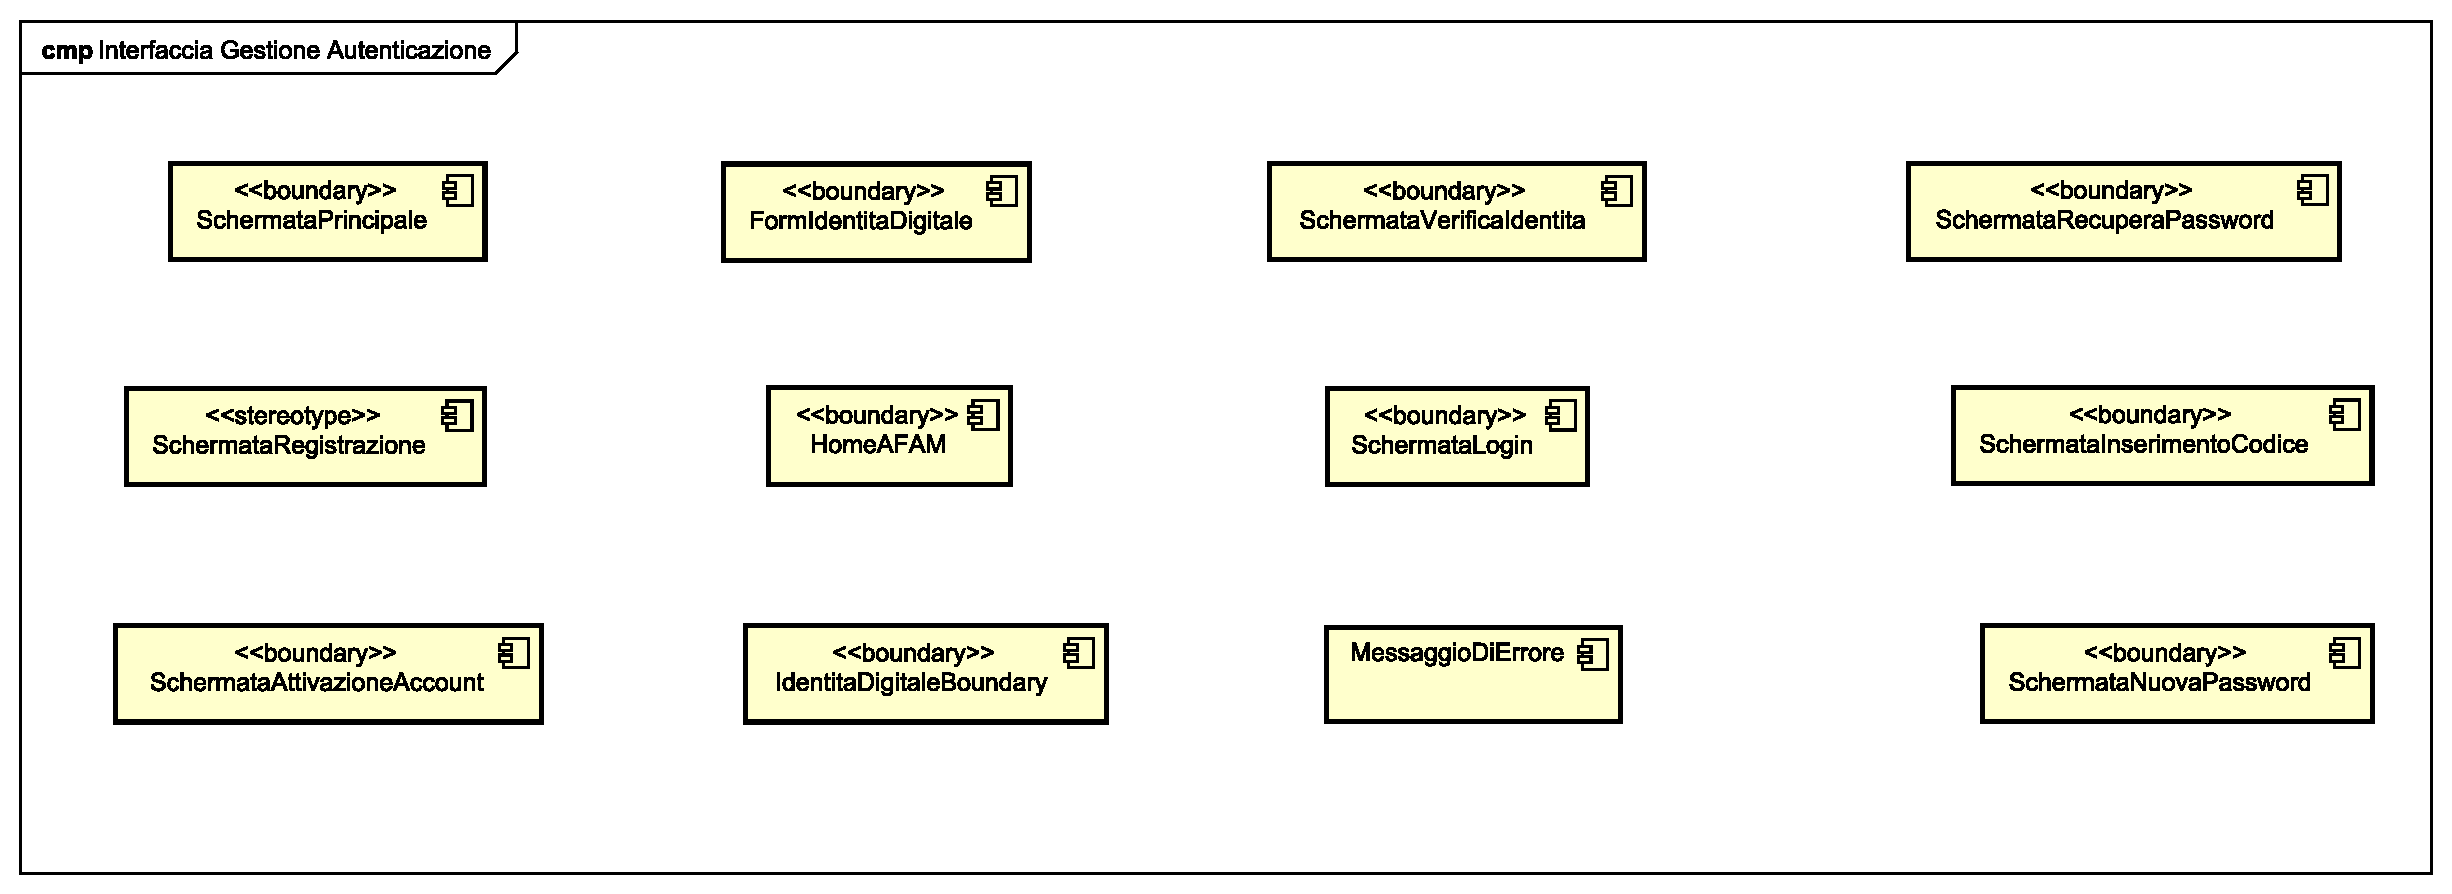
\includegraphics[width=\textwidth,height=0.72\textheight,keepaspectratio]{pdf/asta/gest_aut_Interfaccia_Gestione_Autenticazione.pdf}
    \caption{Interfaccia del sottosistema Gestione Autenticazione}
    \label{fig:interfaccia_gestione_autenticazione}
\end{figure}

\begin{figure}[H]
    \centering
    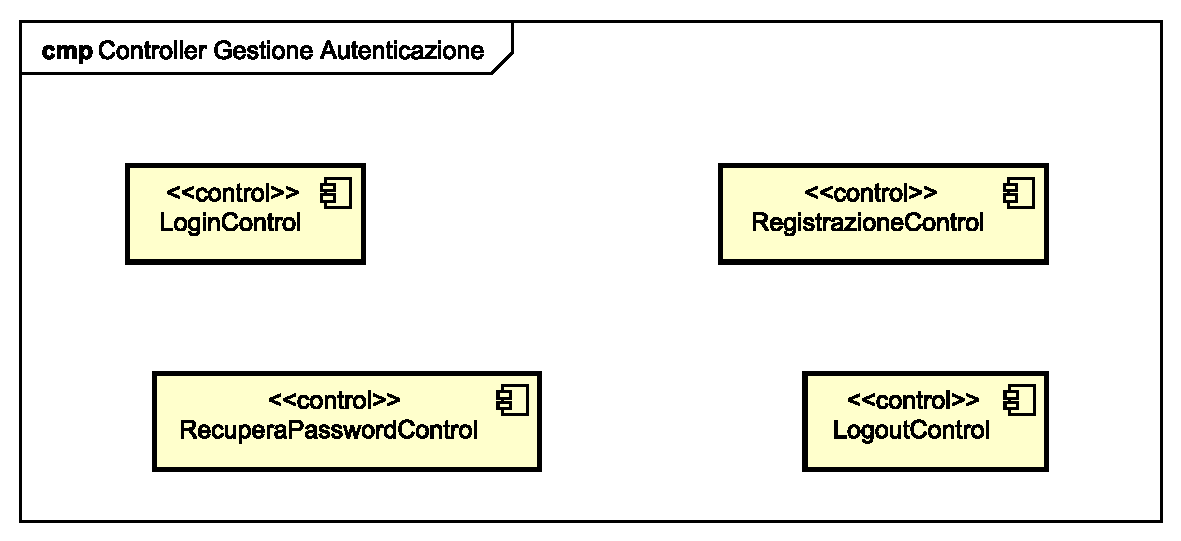
\includegraphics[width=\textwidth,height=0.72\textheight,keepaspectratio]{pdf/asta/gest_aut_Controller_Gestione_Autenticazione.pdf}
    \caption{Controller del sottosistema Gestione Autenticazione}
    \label{fig:controller_gestione_autenticazione}
\end{figure}

\newpage

\textbf{Gestione Condivisione:}

\begin{figure}[H]
    \centering
    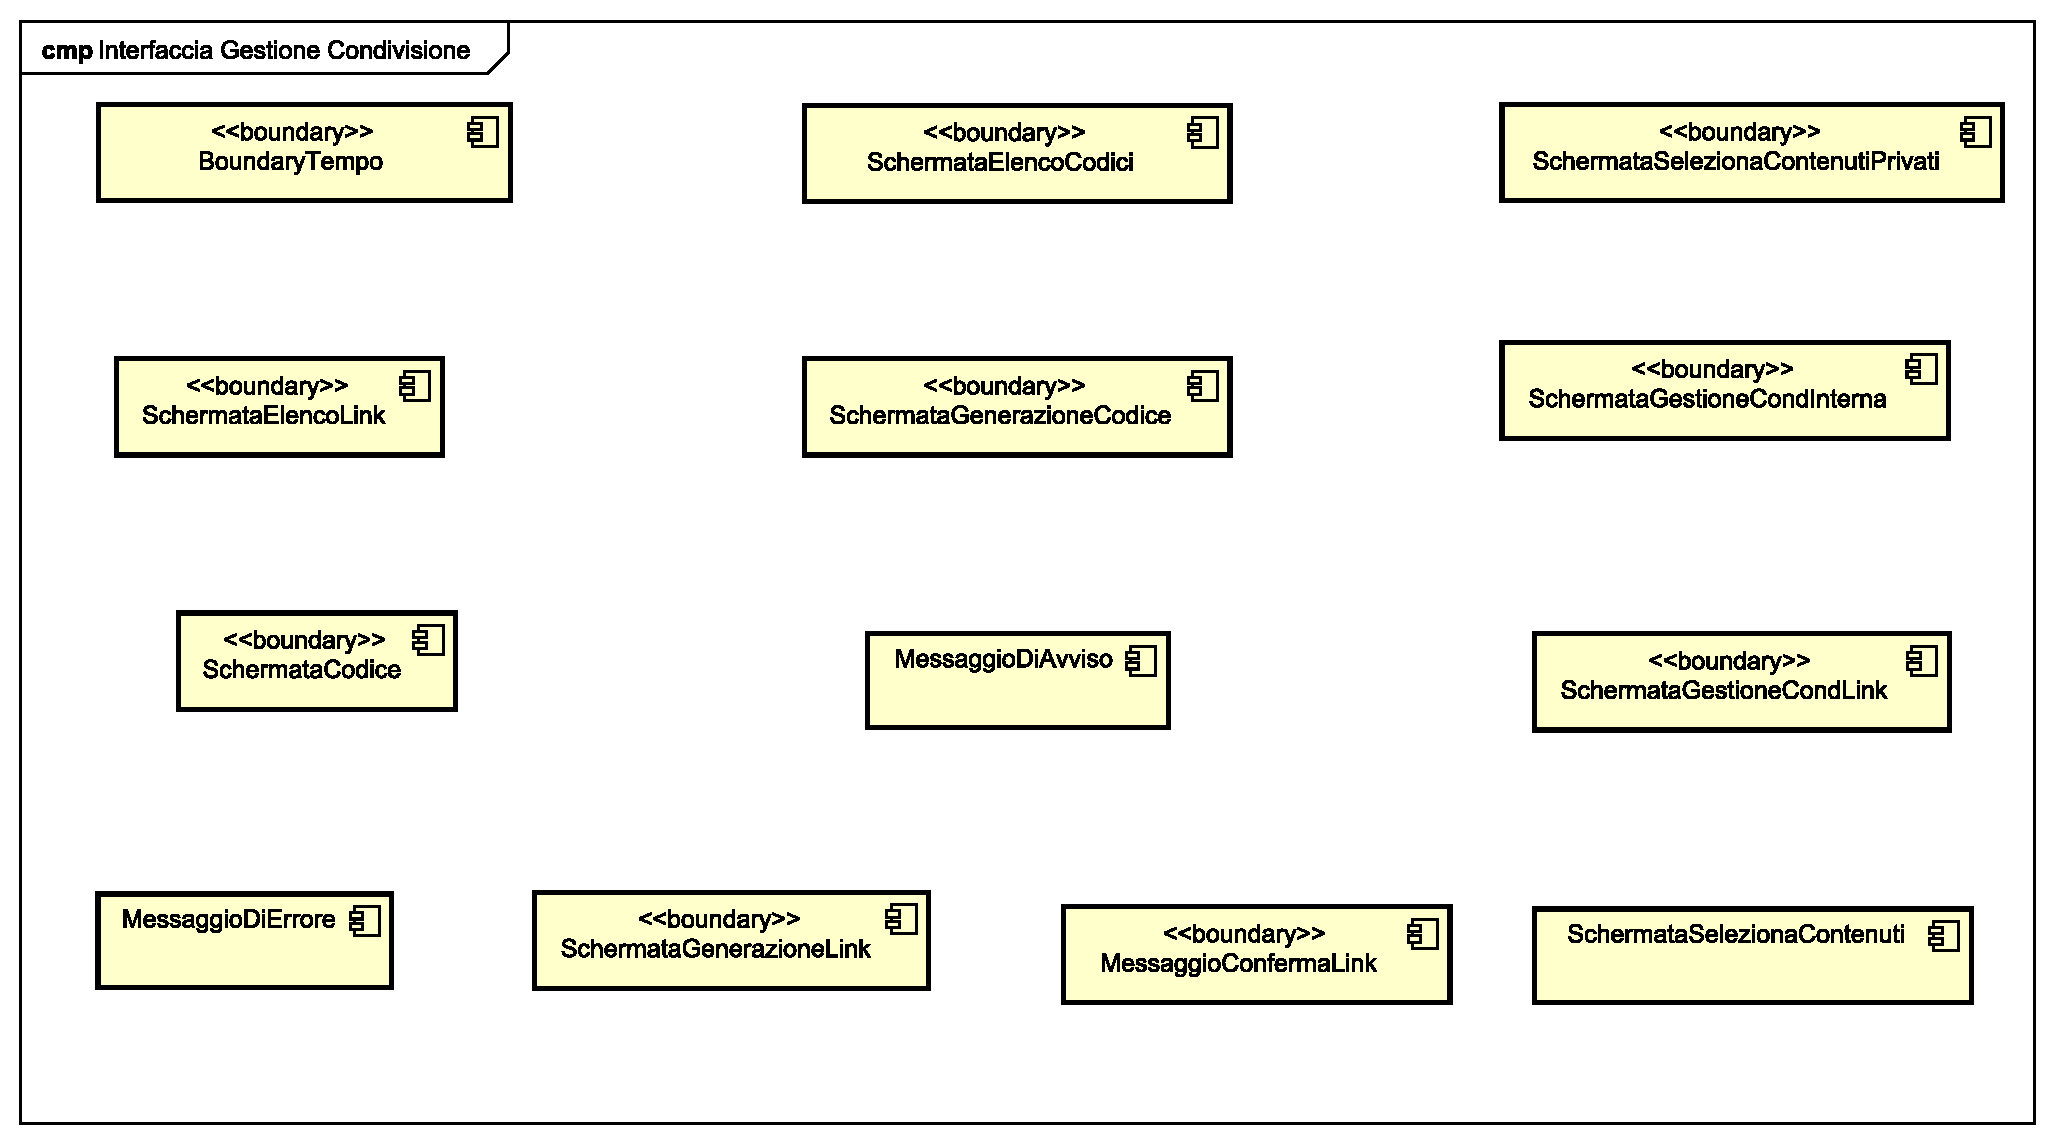
\includegraphics[width=\textwidth,height=0.72\textheight,keepaspectratio]{pdf/asta/gestioneCondivisione_Interfaccia_Gestione_Condivisione_.pdf}
    \caption{Interfaccia del sottosistema Gestione Condivisione}
    \label{fig:interfaccia_gestione_condivisione}
\end{figure}

\begin{figure}[H]
    \centering
    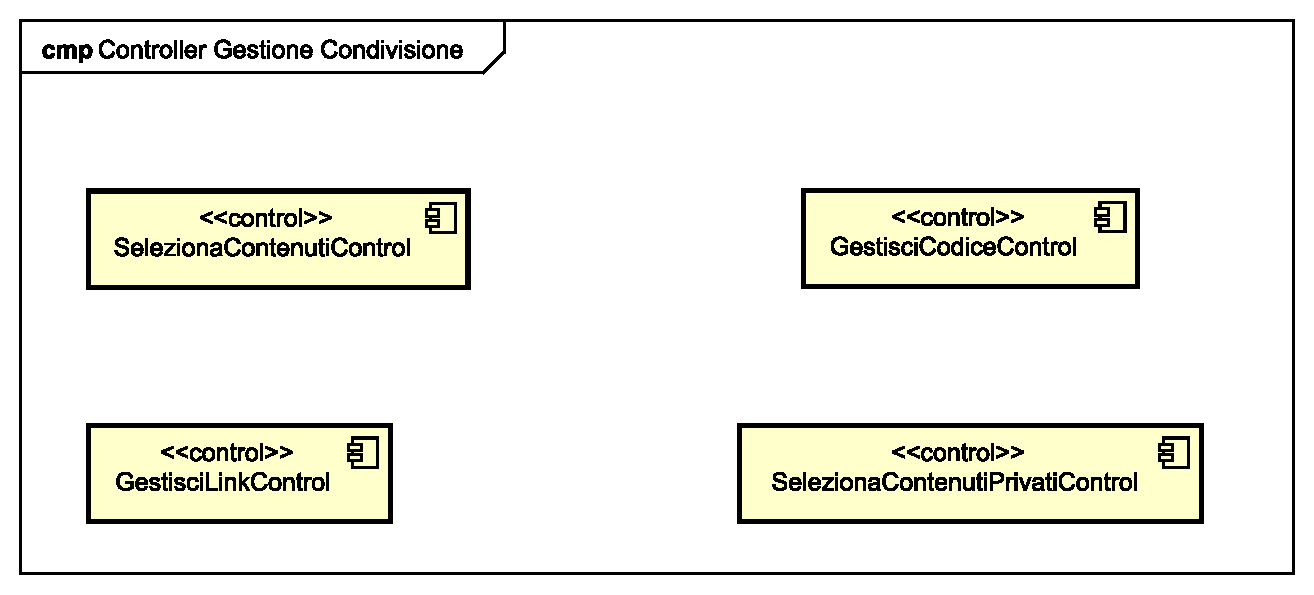
\includegraphics[width=\textwidth,height=0.72\textheight,keepaspectratio]{pdf/asta/gestioneCondivisione_Controller_Gestione_Condivisione_.pdf}
    \caption{Controller del sottosistema Gestione Condivisione}
    \label{fig:controller_gestione_condivisione}
\end{figure}

\newpage

\textbf{Consultazione:}

\begin{figure}[H]
    \centering
    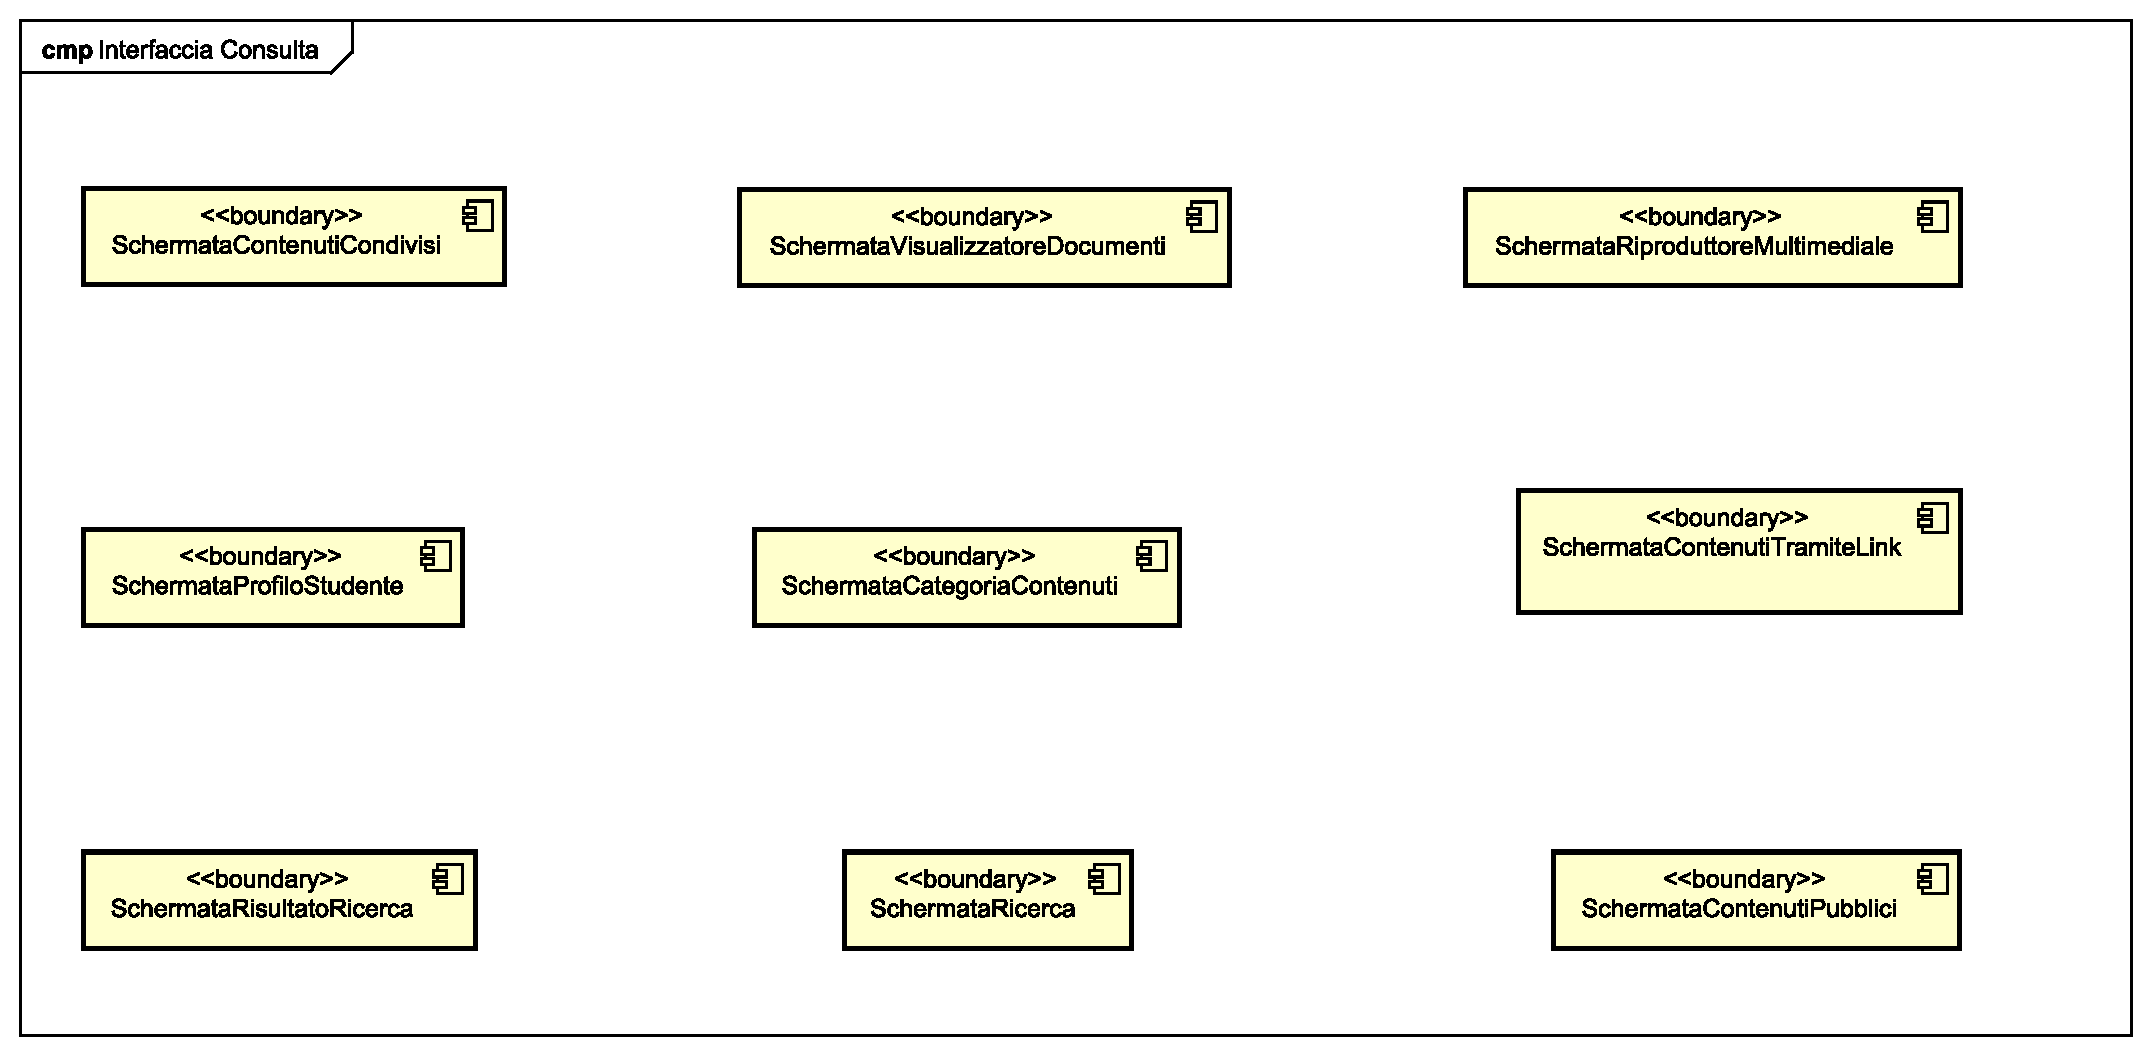
\includegraphics[width=\textwidth,height=0.72\textheight,keepaspectratio]{pdf/asta/consulta_Interfaccia_Consulta_.pdf}
    \caption{Interfaccia del sottosistema Consultazione}
    \label{fig:interfaccia_consultazione}
\end{figure}

\begin{figure}[H]
    \centering
    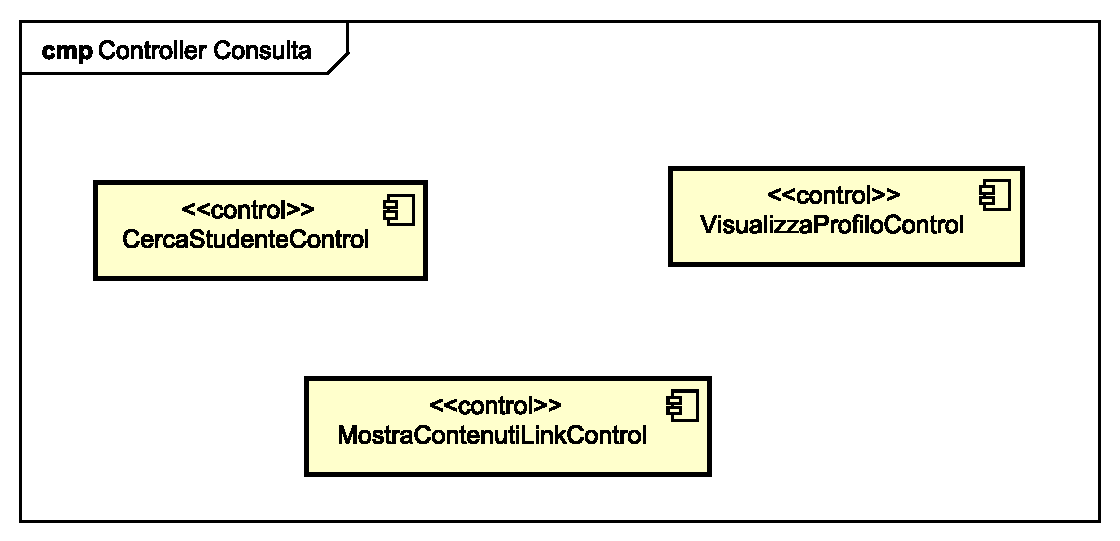
\includegraphics[width=\textwidth,height=0.72\textheight,keepaspectratio]{pdf/asta/consulta_Controller_Consulta_.pdf}
    \caption{Controller del sottosistema Consultazione}
    \label{fig:controller_consultazione}
\end{figure}

\newpage

\textbf{Gestione Operazioni Automatiche:}

\begin{figure}[H]
    \centering
    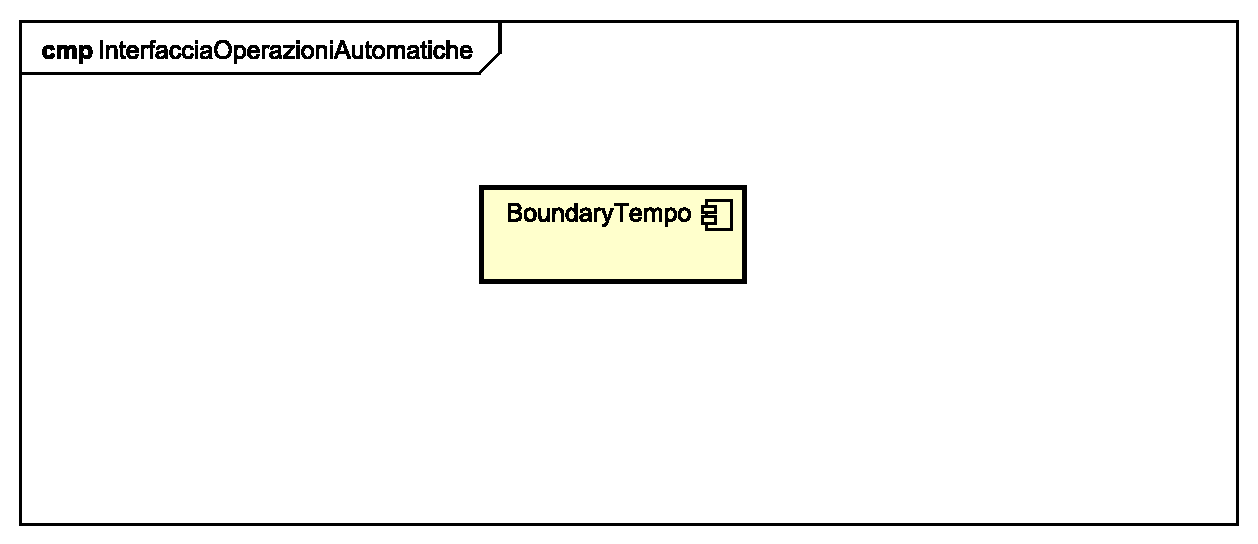
\includegraphics[width=\textwidth,height=0.72\textheight,keepaspectratio]{pdf/asta/gestioneOperazioniAutomatiche_Interfaccia_Operazioni_Automatiche.pdf}
    \caption{Interfaccia del sottosistema Gestione Operazioni Automatiche}
    \label{fig:interfaccia_operazioni_automatiche}
\end{figure}

\begin{figure}[H]
    \centering
    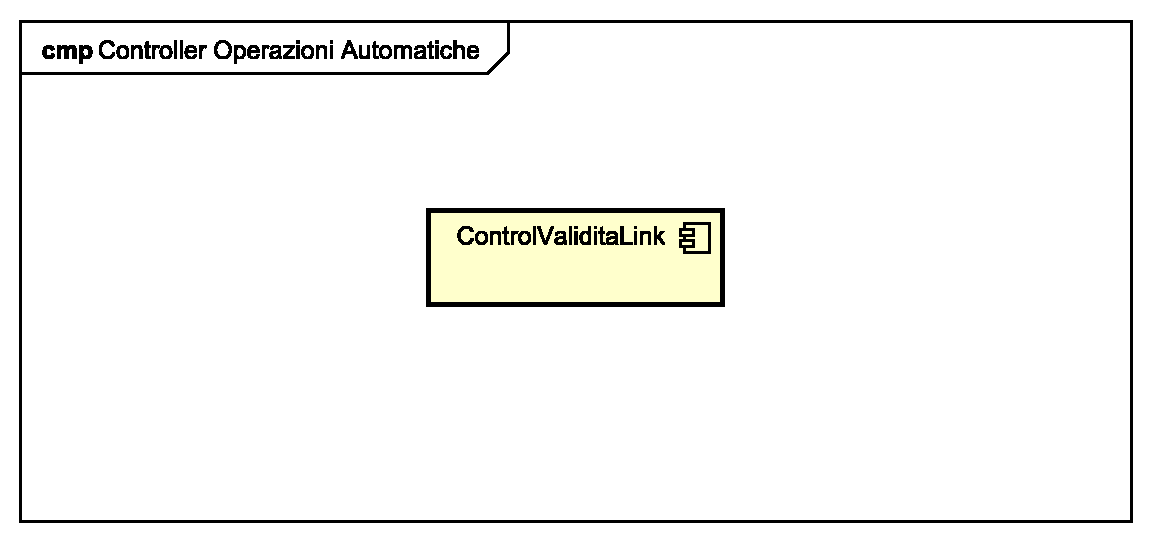
\includegraphics[width=\textwidth,height=0.72\textheight,keepaspectratio]{pdf/asta/gestioneOperazioniAutomatiche_Controller_Operazioni_Automatiche.pdf}
    \caption{Controller del sottosistema Gestione Operazioni Automatiche}
    \label{fig:controller_operazioni_automatiche}
\end{figure}

\newpage

\subsection{Mappatura hardware e software}
\spaziocontenuto

\newpage

\section{Gestione dei dati persistenti}

\subsection{Modello ER}
\spaziocontenuto

\newpage

\subsection{Modello relazionale}
\spaziocontenuto

\newpage

\subsection{Struttura delle tabelle}
\textbf{DBMS:}
\begingroup
\footnotesize
\setlength{\tabcolsep}{3pt}
\renewcommand{\arraystretch}{1.2}

\paragraph{Tabella Studente}
\begin{longtable}{|
>{\columncolor{unipablue}\color{white}\bfseries\raggedright\arraybackslash}p{3.1cm}|
>{\raggedright\arraybackslash}p{3.15cm}|
>{\raggedright\arraybackslash}p{3.45cm}|
>{\raggedright\arraybackslash}p{4.15cm}|}
\hline
\multicolumn{1}{|c|}{\cellcolor{unipablue}\color{white}\textbf{Nome}} &
\multicolumn{1}{c|}{\textbf{Tipo}} &
\multicolumn{1}{c|}{\textbf{Vincoli}} &
\multicolumn{1}{c|}{\textbf{Descrizione}} \\
\hline
id\_studente & INT & PK, AUTO INC., NOT NULL & Identificativo dello studente. \\ \hline
nome & VARCHAR(100) & NOT NULL & Nome anagrafico. \\ \hline
cognome & VARCHAR(100) & NOT NULL & Cognome anagrafico. \\ \hline
codice\_fiscale & CHAR(16) & UNIQUE, NOT NULL & Codice fiscale. \\ \hline
email & VARCHAR(255) & UNIQUE, NOT NULL & Email di accesso. \\ \hline
password & VARCHAR(255) & NOT NULL & Password cifrata/hash. \\ \hline
telefono & VARCHAR(20) & NULL & Recapito telefonico. \\ \hline
\caption{Struttura della tabella Studente}
\label{tab:struttura_studente}
\end{longtable}

\paragraph{Tabella Background\_Artistico}
\begin{longtable}{|
>{\columncolor{unipablue}\color{white}\bfseries\raggedright\arraybackslash}p{3.1cm}|
>{\raggedright\arraybackslash}p{3.15cm}|
>{\raggedright\arraybackslash}p{3.45cm}|
>{\raggedright\arraybackslash}p{4.15cm}|}
\hline
\multicolumn{1}{|c|}{\cellcolor{unipablue}\color{white}\textbf{Nome}} &
\multicolumn{1}{c|}{\textbf{Tipo}} &
\multicolumn{1}{c|}{\textbf{Vincoli}} &
\multicolumn{1}{c|}{\textbf{Descrizione}} \\
\hline
id\_background & INT & PK, AUTO INC., NOT NULL & Identificativo del background. \\ \hline
scuola\_universitaria & VARCHAR(255) & NULL & Istituto frequentato. \\ \hline
collaborazioni & TEXT & NULL & Collaborazioni artistiche. \\ \hline
autori & TEXT & NULL & Autori o riferimenti. \\ \hline
partecipazioni & TEXT & NULL & Eventi e concorsi. \\ \hline
id\_studente & INT & FK, NOT NULL & Studente proprietario. \\ \hline
\caption{Struttura della tabella Background\_Artistico}
\label{tab:struttura_background_artistico}
\end{longtable}

\newpage

\paragraph{Tabella Categoria\_Artistica}
\begin{longtable}{|
>{\columncolor{unipablue}\color{white}\bfseries\raggedright\arraybackslash}p{3.1cm}|
>{\raggedright\arraybackslash}p{3.15cm}|
>{\raggedright\arraybackslash}p{3.45cm}|
>{\raggedright\arraybackslash}p{4.15cm}|}
\hline
\multicolumn{1}{|c|}{\cellcolor{unipablue}\color{white}\textbf{Nome}} &
\multicolumn{1}{c|}{\textbf{Tipo}} &
\multicolumn{1}{c|}{\textbf{Vincoli}} &
\multicolumn{1}{c|}{\textbf{Descrizione}} \\
\hline
id\_categoria & INT & PK, AUTO INC., NOT NULL & Identificativo categoria. \\ \hline
nome\_categoria & VARCHAR(100) & NOT NULL & Nome della categoria. \\ \hline
id\_studente & INT & FK, NOT NULL & Studente proprietario. \\ \hline
\caption{Struttura della tabella Categoria\_Artistica}
\label{tab:struttura_categoria_artistica}
\end{longtable}

\paragraph{Tabella Contenuto\_File}
\begin{longtable}{|
>{\columncolor{unipablue}\color{white}\bfseries\raggedright\arraybackslash}p{3.1cm}|
>{\raggedright\arraybackslash}p{3.15cm}|
>{\raggedright\arraybackslash}p{3.45cm}|
>{\raggedright\arraybackslash}p{4.15cm}|}
\hline
\multicolumn{1}{|c|}{\cellcolor{unipablue}\color{white}\textbf{Nome}} &
\multicolumn{1}{c|}{\textbf{Tipo}} &
\multicolumn{1}{c|}{\textbf{Vincoli}} &
\multicolumn{1}{c|}{\textbf{Descrizione}} \\
\hline
id\_file & INT & PK, AUTO INC., NOT NULL & Identificativo del file. \\ \hline
titolo & VARCHAR(150) & NOT NULL & Titolo del contenuto. \\ \hline
descrizione & TEXT & NULL & Descrizione breve. \\ \hline
formato & VARCHAR(20) & NOT NULL & Tipo del file. \\ \hline
dimensione & INT & NOT NULL & Dimensione in byte. \\ \hline
stato\_privacy & ENUM & NOT NULL & Pubblico o privato. \\ \hline
percorso\_fisico & VARCHAR(255) & NOT NULL & Percorso di storage. \\ \hline
id\_categoria & INT & FK, NOT NULL & Categoria associata. \\ \hline
\caption{Struttura della tabella Contenuto\_File}
\label{tab:struttura_contenuto_file}
\end{longtable}

\newpage

\paragraph{Tabella Link\_Condivisione}
\begin{longtable}{|
>{\columncolor{unipablue}\color{white}\bfseries\raggedright\arraybackslash}p{3.1cm}|
>{\raggedright\arraybackslash}p{3.15cm}|
>{\raggedright\arraybackslash}p{3.45cm}|
>{\raggedright\arraybackslash}p{4.15cm}|}
\hline
\multicolumn{1}{|c|}{\cellcolor{unipablue}\color{white}\textbf{Nome}} &
\multicolumn{1}{c|}{\textbf{Tipo}} &
\multicolumn{1}{c|}{\textbf{Vincoli}} &
\multicolumn{1}{c|}{\textbf{Descrizione}} \\
\hline
id\_link & INT & PK, AUTO INC., NOT NULL & Identificativo del link. \\ \hline
token\_url & VARCHAR(255) & UNIQUE, NOT NULL & Token del link. \\ \hline
data\_creazione & DATETIME & NOT NULL & Data di generazione. \\ \hline
data\_scadenza & DATETIME & NOT NULL & Termine di validita'. \\ \hline
visualizzato & BOOLEAN & NOT NULL, DEFAULT FALSE & Stato di lettura. \\ \hline
stato\_link & ENUM & NOT NULL & Attivo o revocato. \\ \hline
id\_studente & INT & FK, NOT NULL & Studente creatore. \\ \hline
\caption{Struttura della tabella Link\_Condivisione}
\label{tab:struttura_link_condivisione}
\end{longtable}


\paragraph{Tabella Dettaglio\_Link}
\begin{longtable}{|
>{\columncolor{unipablue}\color{white}\bfseries\raggedright\arraybackslash}p{3.1cm}|
>{\raggedright\arraybackslash}p{3.15cm}|
>{\raggedright\arraybackslash}p{3.45cm}|
>{\raggedright\arraybackslash}p{4.15cm}|}
\hline
\multicolumn{1}{|c|}{\cellcolor{unipablue}\color{white}\textbf{Nome}} &
\multicolumn{1}{c|}{\textbf{Tipo}} &
\multicolumn{1}{c|}{\textbf{Vincoli}} &
\multicolumn{1}{c|}{\textbf{Descrizione}} \\
\hline
id\_link & INT & PK, FK, NOT NULL & Link associato. \\ \hline
id\_file & INT & PK, FK, NOT NULL & File condiviso. \\ \hline
\caption{Struttura della tabella Dettaglio\_Link}
\label{tab:struttura_dettaglio_link}
\end{longtable}

\newpage


\paragraph{Tabella Codice\_Sblocco}
\begin{longtable}{|
>{\columncolor{unipablue}\color{white}\bfseries\raggedright\arraybackslash}p{3.1cm}|
>{\raggedright\arraybackslash}p{3.15cm}|
>{\raggedright\arraybackslash}p{3.45cm}|
>{\raggedright\arraybackslash}p{4.15cm}|}
\hline
\multicolumn{1}{|c|}{\cellcolor{unipablue}\color{white}\textbf{Nome}} &
\multicolumn{1}{c|}{\textbf{Tipo}} &
\multicolumn{1}{c|}{\textbf{Vincoli}} &
\multicolumn{1}{c|}{\textbf{Descrizione}} \\
\hline
id\_codice & INT & PK, AUTO INC., NOT NULL & Identificativo codice. \\ \hline
token\_testuale & VARCHAR(100) & UNIQUE, NOT NULL & Codice di sblocco. \\ \hline
stato\_codice & ENUM & NOT NULL & Attivo o revocato. \\ \hline
id\_studente & INT & FK, NOT NULL & Studente creatore. \\ \hline
\caption{Struttura della tabella Codice\_Sblocco}
\label{tab:struttura_codice_sblocco}
\end{longtable}


\paragraph{Tabella Dettaglio\_Codice}
\begin{longtable}{|
>{\columncolor{unipablue}\color{white}\bfseries\raggedright\arraybackslash}p{3.1cm}|
>{\raggedright\arraybackslash}p{3.15cm}|
>{\raggedright\arraybackslash}p{3.45cm}|
>{\raggedright\arraybackslash}p{4.15cm}|}
\hline
\multicolumn{1}{|c|}{\cellcolor{unipablue}\color{white}\textbf{Nome}} &
\multicolumn{1}{c|}{\textbf{Tipo}} &
\multicolumn{1}{c|}{\textbf{Vincoli}} &
\multicolumn{1}{c|}{\textbf{Descrizione}} \\
\hline
id\_codice & INT & PK, FK, NOT NULL & Codice associato. \\ \hline
id\_file & INT & PK, FK, NOT NULL & File sbloccato. \\ \hline
\caption{Struttura della tabella Dettaglio\_Codice}
\label{tab:struttura_dettaglio_codice}
\end{longtable}

\endgroup

\end{document}
